%
% Description -- Verilog-AMS interface
%
% Copyright (C) 2007 Stefan Jahn <stefan@lkcc.org>
%
% Permission is granted to copy, distribute and/or modify this document
% under the terms of the GNU Free Documentation License, Version 1.1
% or any later version published by the Free Software Foundation.
%

\tutsection{Introduction}

Verilog-AMS is a hardware description language.  It can be used to
specify the analogue behaviour of compact device models.  Ususally
these are C or C++ implementations in analogue simulators.  The effort
to implement modern compact models in C/C++ is quite high compared to
the description in Verilog-AMS.

\tutsection{ADMS}

The software ADMS (see \url{http://mot-adms.sourceforge.net}) allows
Verilog-AMS descriptions to be translated into any other programming
language.  It generates a structured XML tree representing the compact
device model description.

\begin{figure}[ht]
\begin{center}
\includegraphics[width=0.8\linewidth]{admsflow}
\end{center}
\caption{ADMS data flow}
\label{fig:admsflow}
\end{figure}
\FloatBarrier

The internal XML tree is used to generate ready-to-compile C or C++
code which is specific to the simulators API.  The code generator is
able to produce
\begin{itemize}
\item evaluation of device equations (current and charge) including
their derivatives,
\item glue code for the simulator API,
\item documentation and
\item any other data described by the original Verilog-AMS input file.
\end{itemize}

\tutsection{XML admst scripts}

The language transformation uses a language named \textbf{admst}.  It
is itself a XML description.  The command line in order to run a
transformation is
\begin{Verbatim}[fontsize=\small]
  $ admsXml <device.va> -e <interface-1.xml> -e <interface-2.xml>
\end{Verbatim}

From version 0.0.11 Qucs comes with the following Verilog-AMS
transformers
\begin{itemize}
\item \verb+qucsMODULEcore.xml+\\
creating the actual analogue simulator implementation
\item \verb+qucsMODULEdefs.xml+\\
creating the parameter descriptions for the analogue simulator
\item \verb+qucsMODULEgui.xml+\\
creating the implementation for the GUI integration
\item \verb+qucsVersion.xml+\\
basic admst library
\item \verb+analogfunction.xml+\\
creating analogue function code
\end{itemize}

In order to create \textbf{admst} scripts for a simulator it is
necessary to understand both, the simulator specific API and how the
ADMS data tree items -- which are based on the Verilog-AMS source file
describing the model -- relate to the API.

\addvspace{12pt}

The command lines for transforming a Verilog-AMS source file into the
appropiate Qucs C++ source files are
\begin{Verbatim}[fontsize=\small]
  $ admsXml <device.va> -e qucsVersion.xml -e qucsMODULEcore.xml
  $ admsXml <device.va> -e qucsVersion.xml -e qucsMODULEgui.xml
  $ admsXml <device.va> -e qucsVersion.xml -e qucsMODULEdefs.xml
  $ admsXml <device.va> -e analogfunction.xml
\end{Verbatim}

each creating an appropriate \verb+*.cpp+ and \verb+*.h+ file.

\addvspace{12pt}

The \textbf{admst} language is used to traverse the internal tree.
The tree's root is defined by the Verilog-AMS module definition.
\begin{lstlisting}[
  language=Verilog,
  xleftmargin=12pt]
module device (node1, node2, ...)
  // module definitions and code
endmodule
\end{lstlisting}

\tutsubsection{Short introduction into the \textbf{admst} language syntax}

Usually the \textbf{admst} language instructions are basically formed
as
\begin{lstlisting}[
  language=XML,
  xleftmargin=12pt,
  morekeywords={admst}]
<admst:instruction argument=...>
  ...
</admst:instruction>
\end{lstlisting}
or
\begin{lstlisting}[
  language=XML,
  xleftmargin=12pt,
  morekeywords={admst}]
<admst:instruction argument=.../>
\end{lstlisting}

Any other text outside these instruction is output to the console or
into an appropriate file.  Some of the most important language
construct are listed below.

\begin{itemize}

\item
Traversing a list: The construct allows to traverse all children of
the selected branch.
\begin{lstlisting}[
  language=XML,
  xleftmargin=12pt,
  morekeywords={admst}]
<admst:for-each select="/module">
  ...
</admst:for-each>
\end{lstlisting}

\item
Defining and using variables: Values from the data tree can be put
into named and typed variables which are then accessible using the \$
operator.
\begin{lstlisting}[
  language=XML,
  xleftmargin=12pt,
  morekeywords={admst}]
<admst:value-of select="name">
<admst:variable name="module" select="%s">
\end{lstlisting}

\item
Opening a file: Printed text (see below) is output into the given
file.
\begin{lstlisting}[
  language=XML,
  xleftmargin=12pt,
  morekeywords={admst}]
<admst:open file="$module.cpp">
  ...
</admst:open>
\end{lstlisting}

\item
Output text: Special characters must be encoded (e.g. \verb+"+ $\rightarrow$
\verb+&quot;+ \verb+<+ $\rightarrow$ \verb+&lt;+ \verb+>+
$\rightarrow$ \verb+&gt+; and \verb+\n+ $\rightarrow$ \verb+\\n+).
\begin{lstlisting}[
  language=XML,
  xleftmargin=12pt,
  morekeywords={admst}]
<admst:text format="This is a text."/>
\end{lstlisting}

\item
Definition of a function:  Functions in \textbf{admst} are called templates.
\begin{lstlisting}[
  language=XML,
  xleftmargin=12pt,
  morekeywords={admst}]
<admst:template match="name_of_function">
  ...
</admst:template>
\end{lstlisting}

\item
Running a function: Templates are applied to part of the internal data
tree.
\begin{lstlisting}[
  language=XML,
  xleftmargin=12pt,
  morekeywords={admst}]
<admst:apply-templates select="date_tree_root_for_function"
                        match="name_of_function"/>
\end{lstlisting}

\item Comments:
\begin{lstlisting}[
  language=XML,
  xleftmargin=12pt,
  morekeywords={admst}]
<!-- this is a comment -->
\end{lstlisting}

\end{itemize}

\tutsubsection{Analogue simulator script}

The analogue simulator implementation consists of several parts.  For
each type of simulation appropriate functions must be implemented.
\begin{itemize}
\item DC simulation\\
\verb+module::initDC (void)+,\\
\verb+module::restartDC (void)+ and\\
\verb+module::calcDC (void)+
\item AC simulation\\
\verb+module::initAC (void)+ and\\
\verb+module::calcAC (nr_double_t)+
\item S-parameter simulation\\
\verb+module::initSP (void)+ and\\
\verb+module::calcSP (nr_double_t)+
\item Transient simulation\\
\verb+module::initTR (void)+ and\\
\verb+module::calcTR (nr_double_t)+
\item AC noise simulation\\
\verb+module::initNoiseAC (void)+ and\\
\verb+module::calcNoiseAC (nr_double_t)+
\item S-parameter noise simulation\\
\verb+module::initNoiseSP (void)+ and\\
\verb+module::calcNoiseSP (nr_double_t)+
\item Harmonic simulation\\
\verb+module::initHB (int)+ and\\
\verb+module::calcHB (int)+
\end{itemize}

These functions go into the \verb+module.core.cpp+ file.  An
appropriate \verb+module.core.h+ header file is also created.

\addvspace{12pt}

In case the Verilog-AMS source file contains analog functions in the
module definition, e.g.
\begin{lstlisting}[
  language=Verilog,
  xleftmargin=12pt]
analog function real name;
  input x;
  real x;
  begin
    name = x * x;
  end
endfunction
\end{lstlisting}

the \verb+analogfunction.xml+ script produces the appropriate C/C++
and header file
\begin{itemize}
\item \verb+module.analogfunction.cpp+
\item \verb+module.analogfunction.h+.
\end{itemize}

The ADMS language transformer is aware of how analogue simlators solve
a network of linear and non-linear devices.  The general
Newton-Raphson algorithm for a DC simulation used in SPICE-like
simulators as well as in Qucs can be expressed as
\begin{equation}
\begin{split}
\label{eq:nonlinearNR}
J^{(m)}\cdot V^{(m+1)} &= J^{(m)}\cdot V^{(m)} - f\left(V^{(m)}\right)\\
&= I_{lin}^{(m)} + I_{nl}^{(m)} - J_{nl}^{(m)}\cdot V^{(m)}
\end{split}
\end{equation}
whereas $J$ denotes the Jacobian
\begin{equation}
J^{(m)} = \left.\dfrac{\partial f\left(V\right)}{\partial V}\right|_{V^{(m)}}
\end{equation}

There are basically two types of contributions supported by ADMS:
currents and charges.  The appropiate Jacobian matrices are
\begin{equation}
J^{(m)} = J_I^{(m)} + J_Q^{(m)} = \underbrace{\left.\dfrac{\partial I\left(V\right)}{\partial V}\right|_{V^{(m)}}}_{\textrm{``static''}} + \underbrace{\left.\dfrac{\partial Q\left(V\right)}{\partial V}\right|_{V^{(m)}}}_{\textrm{``dynamic''}}
\end{equation}
consisting of two real valued matrices $G$
(conductance/transconductance matrix) and $C$
(capacitance/transcapacitance matrix).

\addvspace{12pt}

In the Verilog-AMS desciptions only the current and charge
contributions are mentioned.  The appropriate derivatives are meant to
be automatically formed by the language translator ADMS.
\begin{lstlisting}[
  language=Verilog,
  xleftmargin=12pt]
  I(ci,ei) <+ it;       // current contribtion
  I(si,ci) <+ ddt(Qjs); // charge contribtion
\end{lstlisting}

The right-hand side of eq.~\eqref{eq:nonlinearNR} consists of the
linear and non-linear currents of the network as well as the Jacobian
matrix multiplied by the voltage vector.  Since devices are usually
uncorrelated both parts can be computed directly on a per device
basis.

\tutsubsection{Current limitations of ADMS}

The following section contains some simple examples demonstrating
which Verilog-AMS statements can be successfully handled by ADMS and
which not.

\tutsubsubsection{Example 1}

There was a bug in the \textbf{admst} scripts.  They failed to place
the function calls of analogue functions correctly.  This has been
fixed.

\begin{lstlisting}[
  language=Verilog,
  xleftmargin=12pt]
module diode(a, c);  
  inout a, c;
  electrical a, c;

  analog function real current;
    input is, v;
    begin
      current = is * (exp (v / 26e-3) - 1);
    end
  endfunction

  real Vd;
  real Id;

  analog begin
    Vd = V(a, c);
    Id = current (1e-15, Vd);
    I(a, c) <+ Id;
  end

endmodule
\end{lstlisting}

\tutsubsubsection{Example 2}

It is not allowed to mix current and charge contributions in
assignments.  Mixing both emits wrong C/C++ code.  It accounts the
current to be a charge in this case.

\begin{lstlisting}[
  language=Verilog,
  xleftmargin=12pt]
module diode(a, c);  
  inout a, c;
  electrical a, c;

  real Vd, Id, Is, Cp;

  analog begin
    Is = 1e-15;
    Cp = 1e-12;
    Vd = V(a, c);
    Id = Is * (exp (Vd / 26e-3) - 1);

    // not allowed in ADMS
    I(a, c) <+ Id + ddt(Cp*V(a,c));

    // allowed in ADMS
    I(a, c) <+ Id;
    I(a, c) <+ ddt(Cp*V(a,c));
  end

endmodule
\end{lstlisting}

\tutsubsubsection{Example 3}

The following example is rejected by the \textbf{admst} scripts with
this error message.

\begin{Verbatim}[fontsize=\small]
  [info] admsXml-2.2.4 Oct 18 2006 19:50:46
  [fatal] qucsVersion.xml:1497:admst:if[lhs]: missing node source/insource
\end{Verbatim}

An immediate potential on the right hand side is not allowed embedded
in a function.

\begin{lstlisting}[
  language=Verilog,
  xleftmargin=12pt]
module diode(a, c);  
  inout a, c;
  electrical a, c;

  real Id, Is;

  analog begin
    Is = 1e-15;
    Id = Is * (exp (V(a, c) / 26e-3) - 1);

    // not allowed in ADMS
    I(a, c) <+ Is * (exp (V(a, c) / 26e-3) - 1);

    // allowed in ADMS
    I(a, c) <+ Id;
  end

endmodule
\end{lstlisting}

\tutsubsubsection{Example 4}

Potentials on the left-hand side of contribution assignments are not
allowed.  This kind of assignment emits wrong C/C++ code.

\begin{lstlisting}[
  language=Verilog,
  xleftmargin=12pt]
module diode(a, c);  
  inout a, c;
  electrical a, c;

  real Id, Is;
  real Rp;

  analog begin
    Rp = 1e9;
    Is = 1e-15;
    Id = Is * (exp (V(a, c) / 26e-3) - 1);
    I(a, c) <+ Id;

    // allowed in ADMS
    I(a, c) <+ V(a, c) / Rp;

    // not allowed in ADMS
    V(a, c) <+ I(a, c) * Rp;
  end

endmodule
\end{lstlisting}

\tutsubsection{Code for the GUI integration}

The \textbf{admst} script for the GUI creates files according to its
API.  Basically it produces the list of parameters as well their
descriptions (if available) in a property list.  Additionally the
symbol drawing code is emitted which should be adapted to the devices
requirements.

\begin{figure}[ht]
\begin{center}
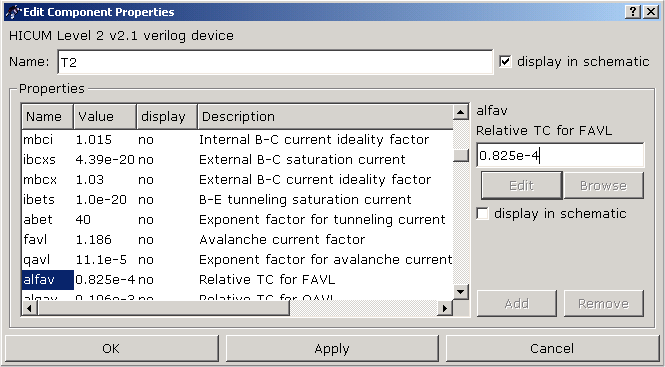
\includegraphics[width=0.9\linewidth]{componentdialog}
\end{center}
\caption{component property dialog in the GUI}
\label{fig:componentdialog}
\end{figure}
\FloatBarrier

In fig.~\ref{fig:componentdialog} the component property dialog of an
implemented device is shown.  In the schematic in
fig.~\ref{fig:hicumschematic} the symbol for the HICUM model is
surrounded with a red circle.  The GUI code is also responsible for
the icons in the listview on the left hand side of the figure.

\begin{figure}[ht]
\begin{center}
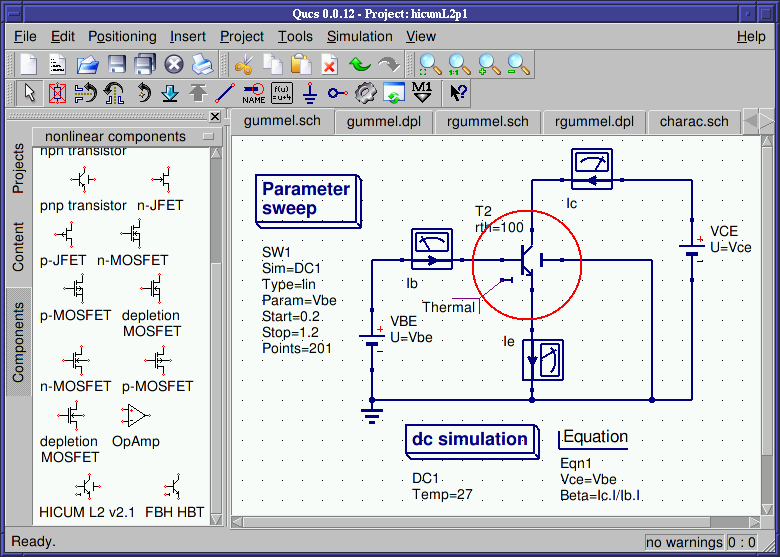
\includegraphics[width=1\linewidth]{hicumschematic}
\end{center}
\caption{schematic with the HICUM transistor symbol}
\label{fig:hicumschematic}
\end{figure}
\FloatBarrier

\tutsection{Adding Verilog-AMS devices to Qucs}

The section gives an overview how to add a Verilog-AMS model to Qucs
in a step-by-step manner.  Be aware that the description is meant for
advanced users partly familiar with the usual GNU/Linux build system
and C/C++ programming.

\tutsubsection{The Verilog-AMS source file}

The starting point of a new Verilog-AMS model in Qucs is the
Verilog-AMS source file which must be aware of the discussed ADMS
limitations.  The example we are going to discuss is a simple diode
model shown in the following listing contained in the
\textbf{diode.va} file.

\begin{lstlisting}[
  language=Verilog,
  xleftmargin=12pt]
`include "disciplines.vams"
`include "constants.vams"

// ADMS specific definitions 
`define attr(txt) (*txt*) 

module diode(a, c);  
  // device terminals
  inout a, c;
  electrical a, c;

  // internal node
  electrical ci;

  // model parameters
  parameter real Is   = 1E-15 from [0:1]
    `attr(info="saturation current");
  parameter real Cp   = 1E-12 from [0:1]
    `attr(info="parallel capacitance");
  parameter real Rs   = 1.0   from (0:inf)
    `attr(info="series resistance");
  parameter real Temp = 300   from (0:inf)
   `attr(info="temperature");

  real Vd, Id, fourkt, twoq, Qp;

  analog begin
    Vd = V(a, ci);
    Id = Is * (exp (Vd / 26e-3) - 1);
    Qp = Cp * Vd;

    I(a, ci) <+ Id;
    I(a, ci) <+ ddt(Qp);
    I(ci, c) <+ V(ci, c) / Rs;

  begin : noise
    fourkt  = 4.0 * `P_K * Temp;
    twoq    = 2.0 * `P_Q;
    I(ci, c) <+ white_noise(fourkt/Rs, "thermal");
    I(a, ci) <+ white_noise(twoq*Id, "shot");
  end // noise

  end // analog

endmodule
\end{lstlisting}

\tutsubsection{Integrating the model into the analogue simulator}

The qucs-core tree of Qucs must be configured using the
--enable-maintainer-mode option.
\begin{Verbatim}[fontsize=\small]
  $ ./configure --enable-maintainer-mode --prefix=/tmp
\end{Verbatim}
Also the software \textbf{adms} must be installed.  It is available at
\url{http://sourceforge.net/projects/mot-adms}.

\addvspace{12pt}

The file \textbf{diode.va} must be copied into the source tree.
\begin{Verbatim}[fontsize=\small]
  $ cp diode.va qucs-core/src/components/verilog/
\end{Verbatim}

In this directory (qucs-core/src/components/verilog/) the Verilog
model can be checked if it can be translated successfully using the
following command lines.
\begin{Verbatim}[fontsize=\small]
  $ admsXml diode.va -e qucsVersion.xml -e qucsMODULEcore.xml
  [info] admsXml-2.2.4 Oct 18 2006 19:50:46
  [info] diode.gui.cpp and diode.gui.h: files created
  [info] elapsed time: 0.0339946
  [info] admst iterations: 4146 (4146 freed)
  $ admsXml diode.va -e analogfunction.xml
  [info] admsXml-2.2.4 Oct 18 2006 19:50:46
  [info] diode.analogfunction.h created
  [info] diode.analogfunction.cpp created
  [info] elapsed time: 0.0262961
  [info] admst iterations: 3919 (3919 freed)
\end{Verbatim}

These command lines create the files for the model evaluation code.
The file names (diode.*) are due to the name of the module contained
in the Verilog-AMS source file.

\addvspace{12pt}

Additionally the source code must be changed in some more locations.
\begin{itemize}
\item \Verb+src/components/component.h+\\
In this file it is necessary to add the line
\begin{Verbatim}[fontsize=\small]
  #include "verilog/diode.core.h"
\end{Verbatim}
\item \Verb+src/components/component_id.h+\\
The file contains unique component identifiers.  It is necessary to
add the Verilog modules name.
\begin{Verbatim}[fontsize=\small]
  enum circuit_type {
    CIR_UNKNOWN = -1,
    ...
    // verilog devices
    CIR_diode,
    ...
  };
\end{Verbatim}
\item \Verb+src/input.cpp+\\
In order to be able to instantiate the new model the file must be
modified as follows.
\begin{Verbatim}[fontsize=\small]
  // The function creates components specified by the type of component. 
  circuit * input::createCircuit (char * type) {
    if (!strcmp (type, "Pac"))
      return new pac ();
    ...
    else if (!strcmp (type, "diode"))
      return new diode ();

    logprint (LOG_ERROR, "no such circuit type `%s'\n", type);
    return NULL;
  }
\end{Verbatim}
\item \Verb+src/qucsdefs.h+\\
Finally the properties including their range definitions must be added
to this file.  The appropiate file can be obtained using the following
command line.
\begin{Verbatim}[fontsize=\small]
  $ admsXml diode.va -e qucsVersion.xml -e qucsMODULEdefs.xml
  [info] admsXml-2.2.4 Oct 18 2006 19:50:46
  [info] diode.defs.h: file created
  [info] elapsed time: 0.0335337
  [info] admst iterations: 4294 (4294 freed)
\end{Verbatim}
The emitted file \textbf{diode.defs.h} looks like
\begin{Verbatim}[fontsize=\small]
  /* diode verilog device */
  { "diode", 2, PROP_COMPONENT, PROP_NO_SUBSTRATE, PROP_NONLINEAR,
    {
      { "Is", PROP_REAL, { 1E-15, PROP_NO_STR }, { '[', 0, 1, ']' } },
      { "Cp", PROP_REAL, { 1E-12, PROP_NO_STR }, { '[', 0, 1, ']' } },
      { "Rs", PROP_REAL, { 1.0, PROP_NO_STR }, { ']', 0, 0, '.' } },
      { "Temp", PROP_REAL, { 300, PROP_NO_STR }, { ']', 0, 0, '.' } },
      PROP_NO_PROP },
    { PROP_NO_PROP }
  },
\end{Verbatim}
representing the parameters defined in the original Verilog-AMS file.
This excerpt must be included in the \textbf{src/qucsdefs.h} file into
this structure:
\begin{Verbatim}[fontsize=\small]
  // List of available components.
  struct define_t qucs_definition_available[] =
  {
    ...
    /* end of list */
    { NULL, 0, 0, 0, 0, { PROP_NO_PROP }, { PROP_NO_PROP } }
  };
\end{Verbatim}
\end{itemize}

Finally the \textbf{Makefile.am} in the
\textbf{src/components/verilog/} directory must be adjusted to make
the build-system aware of the new component.  There must be added
\begin{Verbatim}[fontsize=\small]
  libverilog_a_SOURCES = ... \
          diode.analogfuncction.cpp diode.core.cpp

  noinst_HEADERS = ... \
          diode.analogfuncction.h diode.core.h

  VERILOG_FILES = ... diode.va

  if MAINTAINER_MODE
  ...
  diode.analogfunction.cpp: analogfunction.xml
  diode.analogfunction.cpp: diode.va
          $(ADMSXML) $< -e analogfunction.xml
  diode.core.cpp: qucsVersion.xml qucsMODULEcore.xml
  diode.core.cpp: diode.va
          $(ADMSXML) $< -e qucsVersion.xml -e qucsMODULEcore.xml
  diode.defs.h: qucsVersion.xml qucsMODULEdefs.xml
  diode.defs.h: diode.va
          $(ADMSXML) $< -e qucsVersion.xml -e qucsMODULEdefs.xml
  diode.gui.cpp: qucsVersion.xml qucsMODULEgui.xml
  diode.gui.cpp: diode.va
          $(ADMSXML) $< -e qucsVersion.xml -e qucsMODULEgui.xml
  ...
  else
\end{Verbatim}
in order to create the correct build rules.

\addvspace{12pt}

If everything worked fine then the new Verilog-AMS model is now
completely integrated into the analogue simulator.

\tutsubsection{Integrating the model into the GUI}

Very likely as the qucs-core tree in the previous section also the
qucs tree of must be configured using the --enable-maintainer-mode
option.
\begin{Verbatim}[fontsize=\small]
  $ ./configure --enable-maintainer-mode --prefix=/tmp
\end{Verbatim}

Still in the \textbf{qucs-core/src/components/verilog} directory it is
now necessary to create the C++ code for the GUI using the following
command line.

\begin{Verbatim}[fontsize=\small]
  $ admsXml diode.va -e qucsVersion.xml -e qucsMODULEgui.xml
  [info] admsXml-2.2.4 Oct 18 2006 19:50:46
  [info] diode.gui.cpp and diode.gui.h: files created
  [info] elapsed time: 0.0345217
  [info] admst iterations: 4146 (4146 freed)
\end{Verbatim}

Both the created files \textbf{diode.gui.cpp} and \textbf{diode.gui.h}
should be copied to the \textbf{qucs/qucs/components} directory.

\addvspace{12pt}

Depending on the type of device several changes must be applied to
these files.  The constructor will basically contain the properties of
the device as they are going to occur in the component property dialog
as depicted in fig.~\ref{fig:componentdialog}.  Check these if they
are complete or if some can be left.
\begin{lstlisting}[
  language=C++,
  xleftmargin=12pt]
diode::diode()
{
  Description = QObject::tr ("diode verilog device");

  Props.append (new Property ("Is", "1E-15", false,
    QObject::tr ("saturation current")));
  Props.append (new Property ("Cp", "1E-12", false,
    QObject::tr ("parallel capacitance")));
  Props.append (new Property ("Rs", "1.0", false,
    QObject::tr ("series resistance")));
  Props.append (new Property ("Temp", "300", false,
    QObject::tr ("temperature")));
  ...
}
\end{lstlisting}

The \textbf{diode::info} function should be adapted to meet the
devices requirements.  The \textbf{BitmapFile} should be changed to
represent a correct PNG file in the \textbf{qucs/bitmaps} directory.
Both the \textbf{Name} and the bitmap are going to appear in the
left-hand component tab as shown in fig.~\ref{fig:hicumschematic}.

\begin{lstlisting}[
  language=C++,
  xleftmargin=12pt]
Element * diode::info(QString& Name, char * &BitmapFile,
                      bool getNewOne)
{
  Name = QObject::tr("Diode");
  BitmapFile = "diode";

  if(getNewOne) return new diode();
  return 0;
}
\end{lstlisting}

The \textbf{diode::info\_pnp()} method can be completely deleted.  It
can be necessary for bipolar transistors where two types of devices
could be displayed (npn and pnp type).  The method must also be
deleted from the header file.  Also, in this case, the new diode class
inherits \textbf{Component} instead of \textbf{MultiViewComponent}.

\addvspace{12pt}

The \textbf{diode::createSymbol()} method must be adapted to represent
a valid schematic symbol.  Anyway, the default code can be used as a
template.
\begin{lstlisting}[
  language=C++,
  xleftmargin=12pt]
void diode::createSymbol()
{
  // normal bipolar
  Lines.append(new Line(-10,-15,-10, 15,QPen(QPen::darkBlue,3)));
  Lines.append(new Line(-30,  0,-10,  0,QPen(QPen::darkBlue,2)));
  Lines.append(new Line(-10, -5,  0,-15,QPen(QPen::darkBlue,2)));
  Lines.append(new Line(  0,-15,  0,-30,QPen(QPen::darkBlue,2)));
  Lines.append(new Line(-10,  5,  0, 15,QPen(QPen::darkBlue,2)));
  Lines.append(new Line(  0, 15,  0, 30,QPen(QPen::darkBlue,2)));

  // substrate node
  Lines.append(new Line(  9,  0, 30,  0,QPen(QPen::darkBlue,2)));
  Lines.append(new Line(  9, -7,  9,  7,QPen(QPen::darkBlue,3)));

  // thermal node
  Lines.append(new Line(-30, 20,-20, 20,QPen(QPen::darkBlue,2)));
  Lines.append(new Line(-20, 17,-20, 23,QPen(QPen::darkBlue,2)));  

  // arrow
  if(Props.getFirst()->Value == "npn") {
    Lines.append(new Line( -6, 15,  0, 15,QPen(QPen::darkBlue,2)));
    Lines.append(new Line(  0,  9,  0, 15,QPen(QPen::darkBlue,2)));
  } else {
    Lines.append(new Line( -5, 10, -5, 16,QPen(QPen::darkBlue,2)));
    Lines.append(new Line( -5, 10,  1, 10,QPen(QPen::darkBlue,2)));
  }

  Ports.append(new Port(  0,-30)); // collector
  Ports.append(new Port(-30,  0)); // base
  Ports.append(new Port(  0, 30)); // emitter
  Ports.append(new Port( 30,  0)); // substrate
  Ports.append(new Port(-30, 20)); // thermal node

  x1 = -30; y1 = -30;
  x2 =  30; y2 =  30;
}
\end{lstlisting}

In order to test the component in the GUI it is necessary to modify
some more source code files.
\begin{itemize}
\item \Verb+qucs/qucs.cpp+\\
In this file the new verilog device will be made available to the
component tab.  If a new non-linear device is added then place it here:
\begin{Verbatim}[fontsize=\small]
  pInfoFunc nonlinearComps[] =
    { ... &diode::info, 0};
\end{Verbatim}
\item \Verb+qucs/components/component.cpp+\\
The new verilog device must be loadable in the GUI.  So in the function
\textbf{getComponentFromName()} add this:
\begin{Verbatim}[fontsize=\small]
  Component* getComponentFromName(QString& Line)
  {
    ...
    case 'd' : if(cstr == "iode") c = new diode();
          break;
    ...
    return c;
  }
\end{Verbatim}
\item \Verb+qucs/components/components.h+\\
In the component header file it is necessary to add:
\begin{Verbatim}[fontsize=\small]
  #include "diode.h"
\end{Verbatim}
\end{itemize}

In order to make the build-sytem aware of the new Verilog model the
file \textbf{qucs/components/Makefile.am} must be modified in the
following way.
\begin{Verbatim}[fontsize=\small]
  libcomponents_a_SOURCES = ... \
    diode.gui.cpp

  noinst_HEADERS = ... \
    diode.gui.h
\end{Verbatim}

With these steps the component is now fully integrated into the GUI.  

\tutsection{Implemented devices}

The following sections presents the models already added in Qucs
including some test schematics and simulation results.

\tutsubsection{HICUM/L2 v2.11 model}

The name HICUM was derived from HIgh-CUrrent Model, indicating that
HICUM initially was developed with special emphasis on modelling the
operating region at high current densities which is very important for
certain high-speed applications.

\addvspace{12pt}

The Verilog-AMS source code can be obtained from
\url{http://www.iee.et.tu-dresden.de/iee/eb/hic_new/hic_source.html}.
The model used in Qucs was a bit modified due to some ADMS
limitations.

\addvspace{12pt}

Some schematics have been setup to verify that the model emits
basically the correct output values and the source code translations
worked properly.

\tutsubsubsection{DC simulation}

The setup for the forward Gummel plot is depicted in
fig.~\ref{fig:fgummel}.  The base-emitter voltage is swept ($V_{BE} =
0.2\dots 1.2$) with a constant voltage across the second diode $V_{BC}
= 0$.

\begin{figure}[ht]
\begin{center}
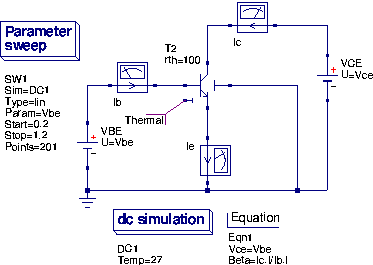
\includegraphics[width=0.7\linewidth]{fgummel}
\end{center}
\caption{forward Gummel plot schematic for HICUM/L2 v2.11 model}
\label{fig:fgummel}
\end{figure}
\FloatBarrier

In fig.~\ref{fig:fgummel_dpl} the logarithmic Gummel plot is shown
including the ratio between the base current and collector current on
the secondary axis.

\begin{figure}[ht]
\begin{center}
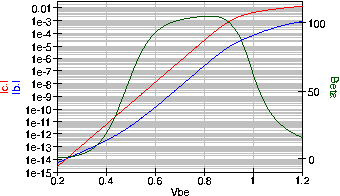
\includegraphics[width=0.8\linewidth]{fgummel_dpl}
\end{center}
\caption{forward Gummel plot for HICUM/L2 v2.11 model}
\label{fig:fgummel_dpl}
\end{figure}
\FloatBarrier

\tutsubsubsection{DC simulation}

In fig.~\ref{fig:charac_sch} the schematic for the output
characteristics of the HICUM model is shown.  The 2-dimensional sweep
describes the function
\begin{equation}
I_C = f\left(V_{CE}, V_{BE}\right)
\end{equation}

\begin{figure}[ht]
\begin{center}
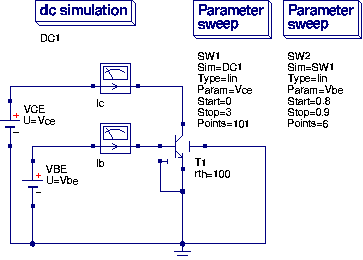
\includegraphics[width=0.7\linewidth]{charac_sch}
\end{center}
\caption{output characteristics schematic for HICUM/L2 v2.11 model}
\label{fig:charac_sch}
\end{figure}
\FloatBarrier

Figure~\ref{fig:charac_dpl} shows the results of the DC simulations
for the output characteristics of the bipolar transistor.

\begin{figure}[ht]
\begin{center}
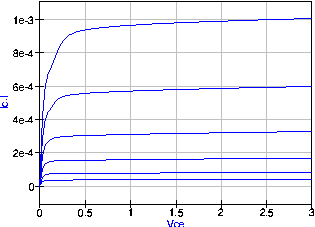
\includegraphics[width=0.6\linewidth]{charac_dpl}
\end{center}
\caption{output characteristics plot for HICUM/L2 v2.11 model}
\label{fig:charac_dpl}
\end{figure}
\FloatBarrier

\tutsubsubsection{AC simulation}

Figures~\ref{fig:acgain_sch} and \ref{fig:acgain_dpl} depict the
schematic and digrams for an AC simulation in a given bias point.  The
current gains magnitude and phase are shown as well as the
characteristics of the small signal base and collector current in the
complex plane (polar plot).

\begin{figure}[ht]
\begin{center}
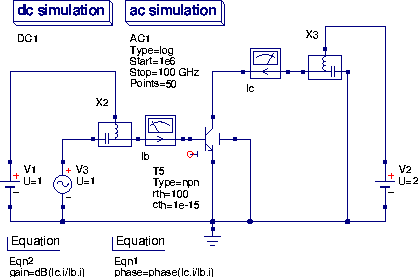
\includegraphics[width=0.7\linewidth]{acgain_sch}
\end{center}
\caption{AC simulation schematic for HICUM/L2 v2.11 model}
\label{fig:acgain_sch}
\end{figure}
\FloatBarrier

\begin{figure}[ht]
\begin{center}
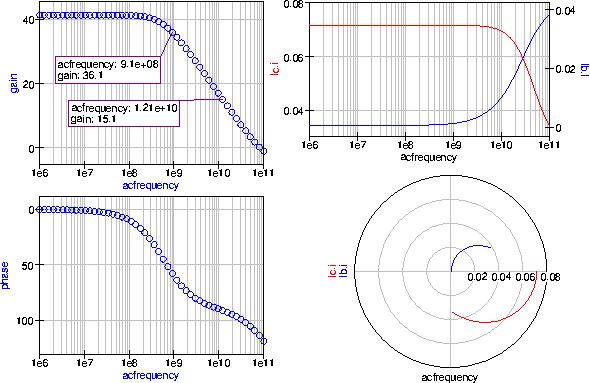
\includegraphics[width=1\linewidth]{acgain_dpl}
\end{center}
\caption{AC simulation plot for HICUM/L2 v2.11 model}
\label{fig:acgain_dpl}
\end{figure}
\FloatBarrier

\tutsubsubsection{S-parameter simulation}

In the figures~\ref{fig:sparam_sch} and \ref{fig:sparam_dpl} a
two-port S-parameter simulation schematic (including noise) as well as
the results are shown.  The four S-parameters are displayed in two
Polar-Smith combi diagrams.  The noise figure as well as the minimal
noise figure are displayed in a logarithmic Cartesian diagram.

\begin{figure}[ht]
\begin{center}
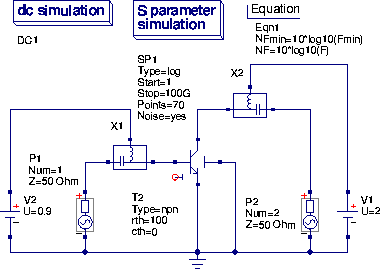
\includegraphics[width=0.7\linewidth]{sparam_sch}
\end{center}
\caption{S-parameter simulation schematic for HICUM/L2 v2.11 model}
\label{fig:sparam_sch}
\end{figure}
\FloatBarrier

\begin{figure}[ht]
\begin{center}
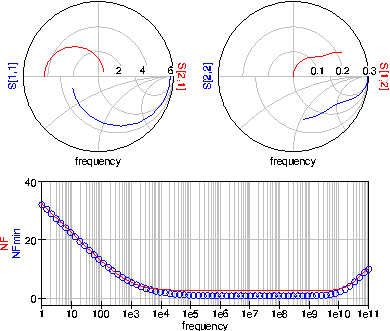
\includegraphics[width=0.8\linewidth]{sparam_dpl}
\end{center}
\caption{S-parameter simulation plot for HICUM/L2 v2.11 model}
\label{fig:sparam_dpl}
\end{figure}
\FloatBarrier

\tutsubsubsection{Transient simulation}

In the schematic in fig.~\ref{fig:transient_sch} a current pulse is
fed into the base of the transistor.  Varying the input capacitance
changes the response in the collector current as shown in
fig.~\ref{fig:transient_dpl}.

\begin{figure}[ht]
\begin{center}
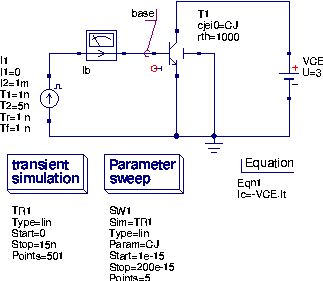
\includegraphics[width=0.6\linewidth]{transient_sch}
\end{center}
\caption{Transient simulation schematic for HICUM/L2 v2.11 model}
\label{fig:transient_sch}
\end{figure}
\FloatBarrier

\begin{figure}[ht]
\begin{center}
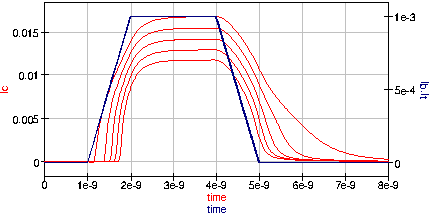
\includegraphics[width=0.8\linewidth]{transient_dpl}
\end{center}
\caption{Transient simulation plot for HICUM/L2 v2.11 model}
\label{fig:transient_dpl}
\end{figure}
\FloatBarrier

\tutsubsection{HBT model by FBH}

The HBT (Hetero Bipolar Transistor) model developed by Matthias
Rudolph at the FBH (Ferdinand Braun Institut f"ur Hochfrequenztechnik)
is available at \url{http://www.designers-guide.org/VerilogAMS}.

\tutsubsubsection{DC simulation}

Forward Gummel plot.

\begin{figure}[ht]
\begin{center}
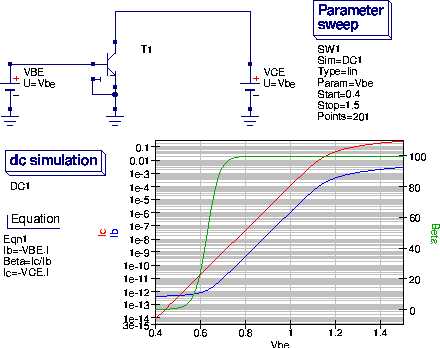
\includegraphics[width=0.9\linewidth]{fbh_fgummel}
\end{center}
\caption{forward Gummel plot schematic for HBT model}
\label{fig:fbh_fgummel}
\end{figure}
\FloatBarrier

\tutsubsubsection{DC simulation}

Output characteristics.

\begin{figure}[ht]
\begin{center}
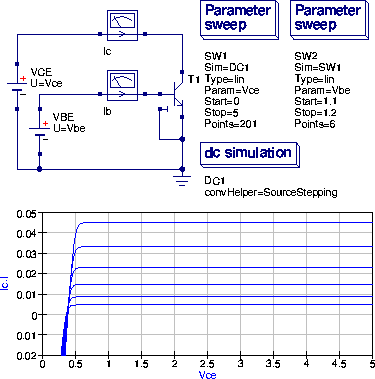
\includegraphics[width=0.7\linewidth]{fbh_charac}
\end{center}
\caption{output characteristics schematic for HBT model}
\label{fig:fbh_charac}
\end{figure}
\FloatBarrier

\tutsection{End Note}
